\section{Evaluation}
\label{sec:Evaluation}
This section contains the evaluation and the graphical representation of the measurements. The following subsections contain the measurement results of the individual tasks listed in chapter \ref{subsec:Measurements}. The measured values are listed in appendix \ref{sec:Measurements}. The aim is to determine the Planck constant. The exact descriptions of the tasks can be found in the assignment \cite{light_quantum}.

%-----------------------------------------------------------------------------------
\subsection{Photoelectric Effect: Direct Measurement}
\label{subsec:Direct_Measurement}
To determine the Planck constant $h$ the software \flqq QtiPlot\frqq\ was used. To calculate the frequency the speed of light $c$ was used. Furthermore, to calculate the Planck constant the elementary charge $e$ was used. The results are shown below:

\[
h/e = (265\pm 9)\cdot 10^{-17}\ \si{V}\cdot\si{s}
\]
\[
h = (424\pm 14)\cdot 10^{-36}\ \si{J}\cdot\si{s}
\]
\[
U_0 = (-841\pm 58)\cdot 10^{-3}\ \si{V}
\]

To obtain these results, linear regression was used on the discrete measured values. The photoelectric voltage was measured directly. This is shown in the following figure \ref{fig:direct}:

\begin{figure}[H]
	\centering
	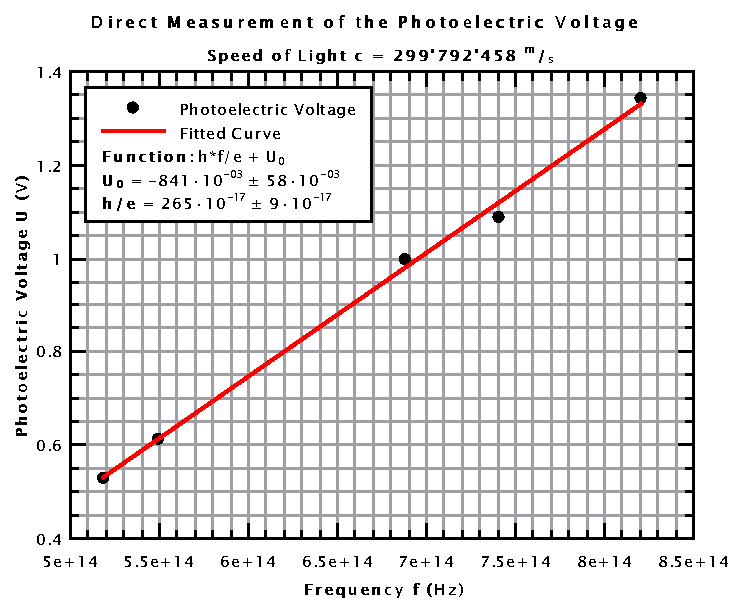
\includegraphics[scale=1]{direct}
	\caption{This plot shows the photoelectric voltage $U$ in function of the frequency $f$. Linear regression was used on the discrete measurement values to obtain $h/e$. An additional voltage offset $U_0$ was added to obtain the in red shown fitted curve. To calculate the frequency $f$ from the wave length $\lambda$, the speed of light $c$ was used (see equation \ref{eq:wave_length_frequency}). The offset voltage $U_0$ is negative.}
	\label{fig:direct}
\end{figure}

\newpage
%-----------------------------------------------------------------------------------
\subsection{Photoelectric Effect: Counter-Field Method}
\label{subsec:Counter-Field_Method}
The Planck constant was also determined by using the counter-field method. The evaluation was carried out in the same way as the last one. The obtained results are shown below:

\[
h/e = (339\pm 32)\cdot 10^{-17}\ \si{V}\cdot\si{s}
\]
\[
h = (544\pm 51)\cdot 10^{-36}\ \si{J}\cdot\si{s}
\]
\[
U_0 = (-1.37\pm 0.22)\ \si{V}
\]

Figure \ref{fig:counter} shows the measured values and the linear fit. This time the photoelectric voltage was not measured directly. The counter-field method was used to obtain the discrete measurement values.

\begin{figure}[H]
	\centering
	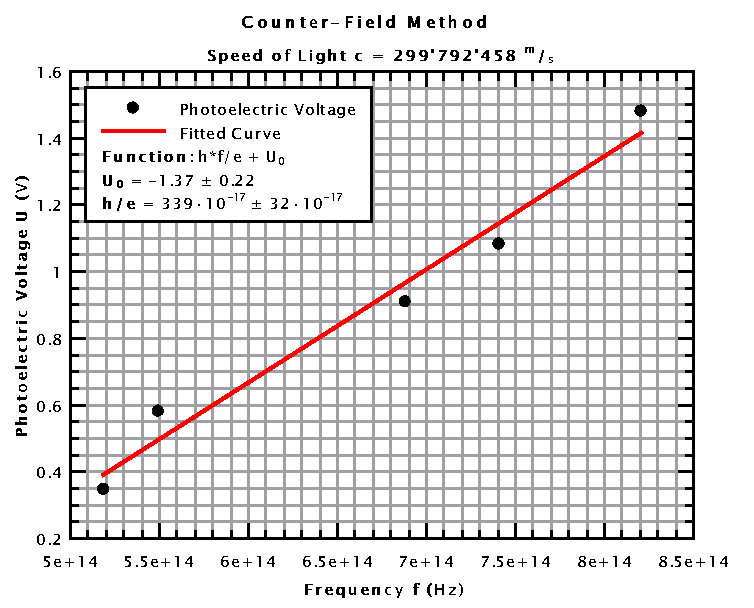
\includegraphics[scale=1]{counter}
	\caption{Measurement values of the photoelectric voltage $U$ in function of the frequency $f$. The photoelectric voltage $U$ was not measured directly. The counter-field method was used. A linear fit (red) was used to obtain $h/e$. The measurement values differ quite a bit from there supposed position on the fitted curve. The offset voltage $U_0$ is even more negative than before.}
	\label{fig:counter}
\end{figure}

\newpage
%-----------------------------------------------------------------------------------
\subsection{Light-Emitting Diode: Threshold Voltage}
\label{subsec:LED_Threshold_Voltage}
To determine the Planck constant, the threshold voltage $U$ and the wave length $\lambda$ of six different LEDs was measured. While it is relatively easy to get an accurate reading of the wave length $\lambda$, it is not easy to get a good reading of the threshold voltage $U$. This can clearly be seen in figure \ref{fig:leds}. Nevertheless, the obtained results are shown below:

\[
h/e = (478\pm 64)\cdot 10^{-17}\ \si{V}\cdot\si{s}
\]
\[
h = (766\pm 103)\cdot 10^{-36}\ \si{J}\cdot\si{s}
\]
\[
U_0 = (-0.25\pm 0.35)\ \si{V}
\]

Linear regression was used again, to obtain a linear fit. The uncertainty of the fit is quite high, since the voltage values are probably off by quite a bit.

\begin{figure}[H]
	\centering
	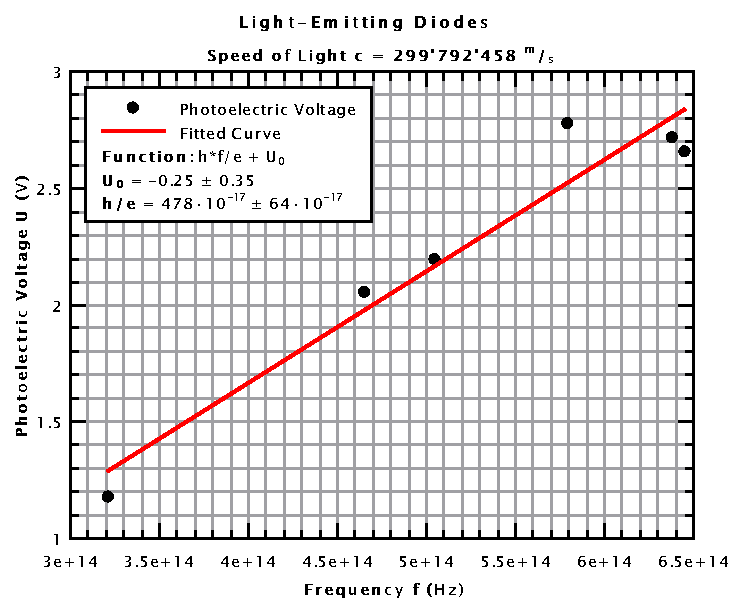
\includegraphics[scale=1]{leds}
	\caption{This plot shows the measured threshold voltage $U$ in function of the frequency $f$. Just like before, linear regression was used on the discrete measurement values to obtain $h/e$. Especially the measurement values with a high frequency $f$ (low wave length $\lambda$) are off by a lot. This is due to the fact, that it is very hard to determine the threshold voltage $U$ accurately. The linear fitted curve is shown in red.}
	\label{fig:leds}
\end{figure}

Figure \ref{fig:dso} shows how the threshold voltage $U$ was determined with an oscilloscope for the infrared LED. The UI characteristic curve was created by using the XY time mode. Figure \ref{fig:spectrum} shows an export from the \flqq Logger Pro\frqq\ software. The wave length $\lambda$ was determined by finding the intensity peak and then reading the wave length $\lambda$ value.

\newpage
%-----------------------------------------------------------------------------------
\begin{figure}[H]
	\centering
	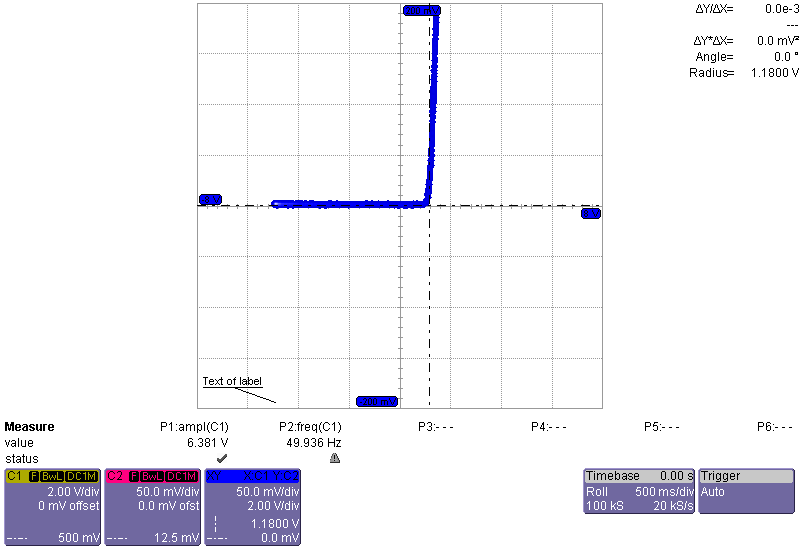
\includegraphics[width=\textwidth]{dso}
	\caption{This is a screenshot of a measurment from the oscilloscope. The threshold voltage was determined with the cursors. In this example the threshold voltage $U$ of the infrared LED was measured and resulted in 1.18 V. The other five measurements were performed in the same way.}
	\label{fig:dso}
\end{figure}

\begin{figure}[H]
	\centering
	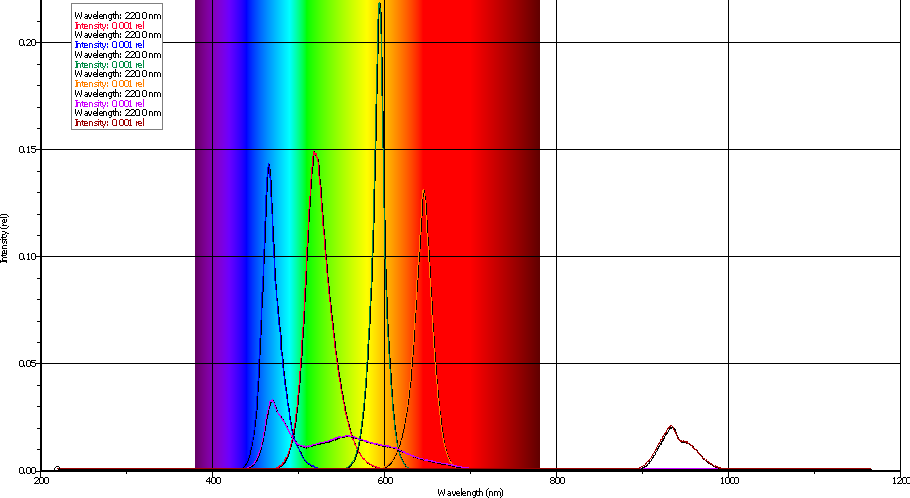
\includegraphics[width=\textwidth]{spectrum}
	\caption{This is an exported graphic from the \flqq Logger Pro\frqq\ software. It shows the measured wave lengths $\lambda$ for the six different LEDs. The four curves with the high peaks are the blue, green, yellow and red LEDs. The peak far right is the infrared LED and the curve with essentially two peaks (quite flat curve) is the white LED.}
	\label{fig:spectrum}
\end{figure}
